\subsection{Parameter identification}

At the first phase, the scheduling system must be robust enough to be put into operation with possibly little a priori information available. A fast revision of the construction conditions of the hotel motivates thence to the use of an initial model estimate of the linear time invariant form \ref{eq:model}. This assumption is not inadequate at all given that the fundamental frequencies of the transference relationships are expected to be low. 

However, it is required that the system acquires a good estimate on the real thermal performance of the building with time. An intelligent layer capable of learning the parameters characterizing its thermal isolating quality is then proposed.  Consider an extended continuous abstraction of the form:

\begin{align*}
& c_i\dot{T}_{i}=-K_{i,e}(T_{i}-T_{e})+\sum_{i\sim j}(T_{i}-T_{j})+K_{u}u_{i}+q^S_{i}\\
& \forall i \mid 0=1...n_r \numberthis
\end{align*}

with parameters $c_i$ (conservation of energy) and transmittance (principle of continuity) parameters for inner adjacencies $K_{i,j}$ as well as those with the exterior (exogenous in nature) state $T_e$. Strictly adjacent rooms $i$ and $j$ are considered by emphasizing the coherence of their flux equality relations, described strictly by $q_{i,j}=K_{i,j}(T_i-T_j)$. Room control inputs $u_i$ are also taken into account as well as the predictable solar flux $q^S_{i}$ radiated into windows of each room. The characteristic discretisation is therefore given by the predictive form  \textbf{$S_p$}:
\begin{align*}
& \hat{T}_{i,t+1}=\frac{1}{c_i}\left[\sum_{i\sim j\bigcup e}(\hat{T}_{i,t}-\hat{T}_{j,t})+K_{u}u_{i,t}+q^S_{i,t}+\hat{T}_{i,t}\right]\\
& u_{i,t}=u_{i,t-1}+K_{u,i}(e_{i,t}-e_{i,t-1})\\
& e_{i,t} = T_{sp,t}-T_{i,t}\\
& \forall i \mid 0=1...n_r\\
& \forall t \mid t=1...P \numberthis
\end{align*}

where already the exterior node is considered inside the whole set of adjacencies per room and a deliberate proportional control structure of the form $q_{u,i}=K_{u,i}(T_{sp,t}-T_i)$ is proposed for $T_sp$ desired temperature at the time a room is to be heated. A pure algebraic error state $e_{i,t}$ is also expanded determining the whole discretisation strategy. 
With initial parameter estimates $K_{i,j}^o$ and $c_{i}^o$ from mechanical abstraction in Eq.~\ref{eq:model}, it is possible to solve a Nonlinear Least Squares optimisation problem with the aim of minimising predicting errors by means of the formulation

 \begin{equation}
 \begin{array}{rlclcl}
 \displaystyle \theta^*=\arg \min_{\theta\in\mathbb{R}} & \multicolumn{3}{l}{(T_{i,t}-\hat{T}_{i,t})^2} \\
 \textrm{s.t.} & \theta \geq 0 \\
 & S_p = 0\\
 \end{array}
 \label{eq:opt_k_cluster}
 \end{equation}

returning the optimal parameter vector $\theta^*$ and performed over timespan $P$. Notice that one can warm up the optimisation routine with an initial first Linear Least Squares approach applied to an ARX-Model attempt. Nevertheless, in the scope of this work, it was demonstrated that the default trust-region-reflective algorithm implemented by \textbf{\texttt{MATLAB}} \texttt{lsqnonlin} solver could deal very well with this task.

For changes in the sampling rate at which the system can learn the parameters of the building, one could also start with a rough approximation and iteratively decrease the time differential in order to refine the solution. The analysis proposed here uses a sampling period of one hour and involves the use of more accurate simulations from the toolbox \textbf{\texttt{E-plus}}, providing the exogenous inputs of the optimisation problem and thence bounding the performance of the system up to the degree of mismatch of the toolbox itself.

In the real scenario, after put in operation, the scheduling system can be interfaced with the (probably) existing thermostats of the building and program itself e.g. once a week to improve the parametric estimation of the real structure and ensure more accurate results with time. Fig.~\ref{fig:sys_id} shows the obtained estimation.

   \begin{figure}[thpb]
   	\centering
   	\framebox{\parbox{3in}{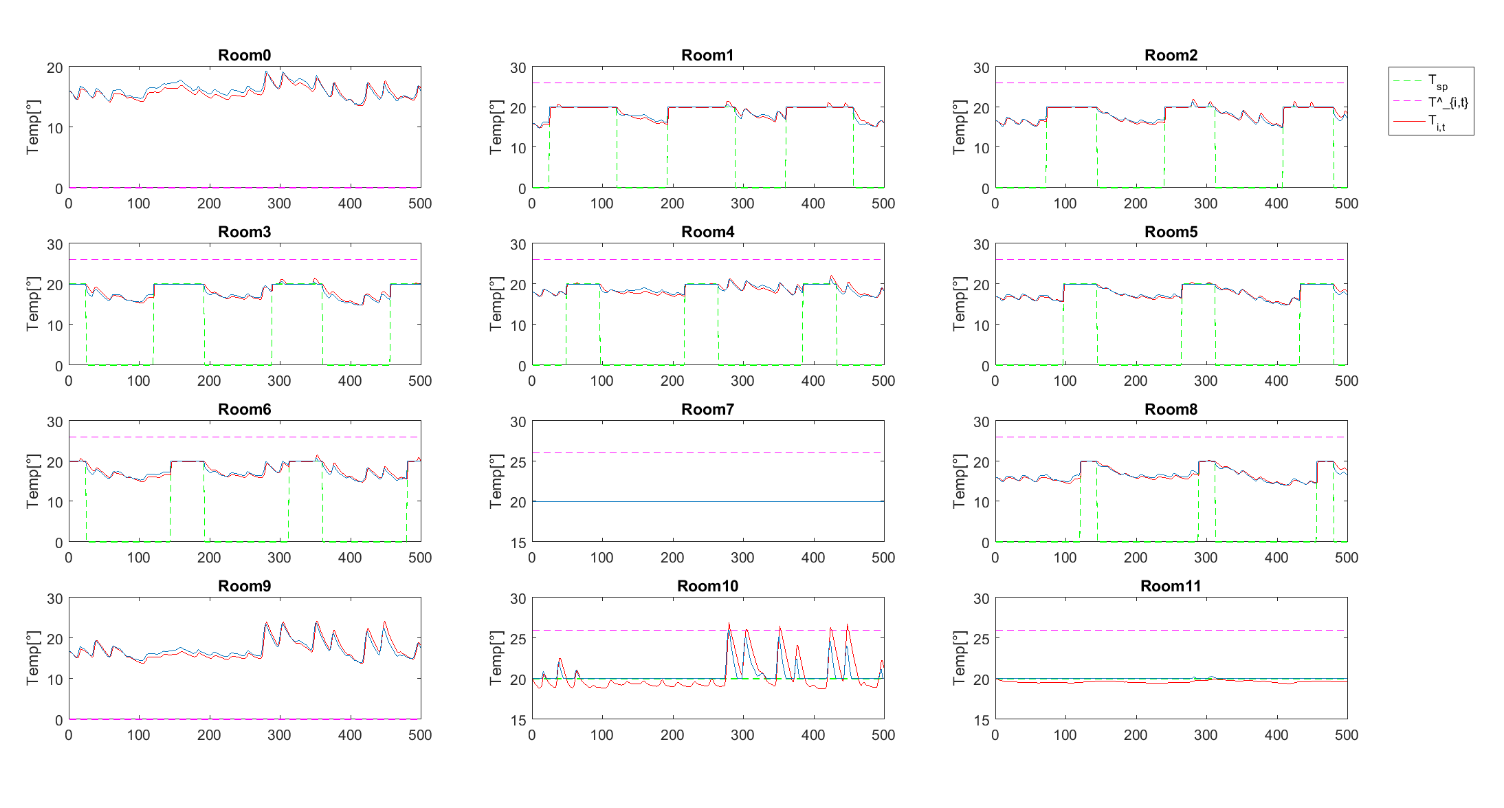
\includegraphics[width=77mm]{img/Sys_ID.png}}}
   		%\includegraphics[scale=1.0]{figurefile}
   		\caption{Forward simulation of the system after parameter identification.}
   		\label{fig:sys_id}
   	\end{figure}

